\documentclass[11pt]{article}

\usepackage[a4paper,margin=1in]{geometry}
\usepackage[T1]{fontenc}
\usepackage[utf8]{inputenc}
\usepackage{ebgaramond}      % match the web version's typeface
\usepackage{textalpha}       % individual Greek letters under pdflatex (\textalpha etc.), full LGR coverage
\usepackage{booktabs}
\usepackage{graphicx}
\usepackage{amsmath}
\usepackage{microtype}
\usepackage[hidelinks]{hyperref}
\usepackage{enumitem}
\setlist{nosep,leftmargin=1.4em}

% --- helpers for the few Greek words we cite (built from textgreek glyphs) ---
% itacism vowels: eta iota upsilon epsilon-iota omicron-iota
\newcommand{\itac}{\texteta, \textiota, \textupsilon, \textepsilon\textiota, \textomicron\textiota}
% visual minuscule confusions
\newcommand{\visconf}{\textgamma/\texttau, \textlambda/\textmu, \textbeta/\textnu, \textrho/\textpi}
\newcommand{\postvoc}{\textbeta/\textupsilon}
% example word pairs
\newcommand{\tais}{\texttau\textalpha\textiota\textfinalsigma}
\newcommand{\tois}{\texttau\textomicron\textiota\textfinalsigma}
\newcommand{\tis}{\texttau\textiota\textfinalsigma}
\newcommand{\ois}{\textomicron\textiota\textfinalsigma}

\title{\vspace{-2em}Teaching Logion How Scribes Actually Slip:\\
\large A Weighted Edit Distance for Byzantine Greek Emendation}
\author{Reza Ramji}
\date{Extends Logion (Cowen-Breen, Brooks, Graziosi, Haubold; \emph{ACL ALP-2023})}

\begin{document}
\maketitle

\begin{abstract}
\noindent Princeton's Logion is a BERT-based model that flags likely scribal errors in
premodern Greek and proposes corrections. To decide which spellings count as
plausible alternatives, it uses classical Levenshtein distance, which treats
every single-character substitution as equally costly. That assumption is wrong
for Byzantine Greek, where a small set of phonetic and visual confusions causes
most copying errors. Replacing the binary distance-1 filter with a
\emph{weighted} Levenshtein neighborhood --- substitution costs drawn from
documented confusion classes --- gives a statistically significant gain on real
attested manuscript variants: top-5 recovery of $42.3\%$ versus a baseline of
$35.7\%$ on $333$ loci from the SBLGNT apparatus (paired McNemar
$p < 10^{-3}$). Two other tested components are inert or harmful, so the winning
configuration is the simple one: weighted Levenshtein on, everything else off.
\end{abstract}

\section{What Logion does}

Ancient Greek survives through centuries of hand-copying, and the copies are full
of errors: smudged letters, dropped words, sounds misheard from dictation.
Logion is a language model (a BERT fine-tuned on premodern Greek) that reads a
passage, flags positions where the transmitted word looks wrong, and proposes
the word it thinks belongs there. Editors use it as a second reader.

For each word it computes a \emph{chance-correction ratio}: how probable is the
word actually written, compared with the most probable near-spelling the model
can substitute in context? Words whose written form is far less probable than an
available alternative are surfaced for expert review. Building that set of
``near-spellings'' requires a notion of which words count as close, and for this
Logion uses \textbf{edit distance} (Levenshtein): the number of single-character
changes that turn one word into another.

\section{The problem: every substitution costs the same}

Classical edit distance is blunt. Changing one letter to \emph{any} other letter
costs exactly one, whether the two are routinely confused or wholly unrelated.
Logion's original filter is blunter still: a yes/no gate that admits any
vocabulary word within distance~1 and weights them all equally.

Real copying errors are not uniform. In Byzantine Greek a handful of confusions
dominate:
\begin{itemize}
  \item \textbf{Itacism} --- \itac{} all came to be pronounced /i/, so scribes
  writing from dictation swapped them constantly. This is the single largest
  source of error.
  \item \textbf{Visual look-alikes} in minuscule script --- \visconf{} are easy
  to misread.
  \item \textbf{Post-vocalic} \postvoc{} --- a sound shift that bled into
  spelling.
\end{itemize}
A metric that treats \texteta${\to}$\textiota{} the same as
\texteta${\to}$\textxi{} discards exactly the signal that matters.

\section{The change: weight the substitutions}

Instead of a yes/no gate, give each substitution a \emph{cost} taken from
documented confusion classes (Allen, \emph{Vox Graeca}; West, \emph{Textual
Criticism}; Reynolds \& Wilson, \emph{Scribes \& Scholars}). Easily-confused
letters cost little; unrelated letters cost the full amount. The filter becomes a
continuous weight rather than a hard cutoff. An itacism swap such as
\tais{}\,/\,\tois{} costs $0.35$ and receives about $3.7\times$ the weight of an
unrelated same-distance edit such as \tis{}\,/\,\ois{}, which costs the full
$1.00$.

\section{Result}

The fairest test uses \textbf{real attested variants}: $333$ loci in the SBLGNT
apparatus where the manuscripts genuinely disagree, i.e. errors real scribes
actually made rather than artificial ones. There the weighted filter recovers
more of them.

\begin{quote}
\textbf{Top-5 recovery: $42.3\%$ vs.\ $35.7\%$ baseline} (paired McNemar
$p < 10^{-3}$). The weighted filter recovered $28$ loci the baseline missed and
lost only $6$. Top-1 trends positive but is not significant
($16.5\%$ vs.\ $14.4\%$, $p = 0.30$).
\end{quote}

\begin{figure}[h]
  \centering
  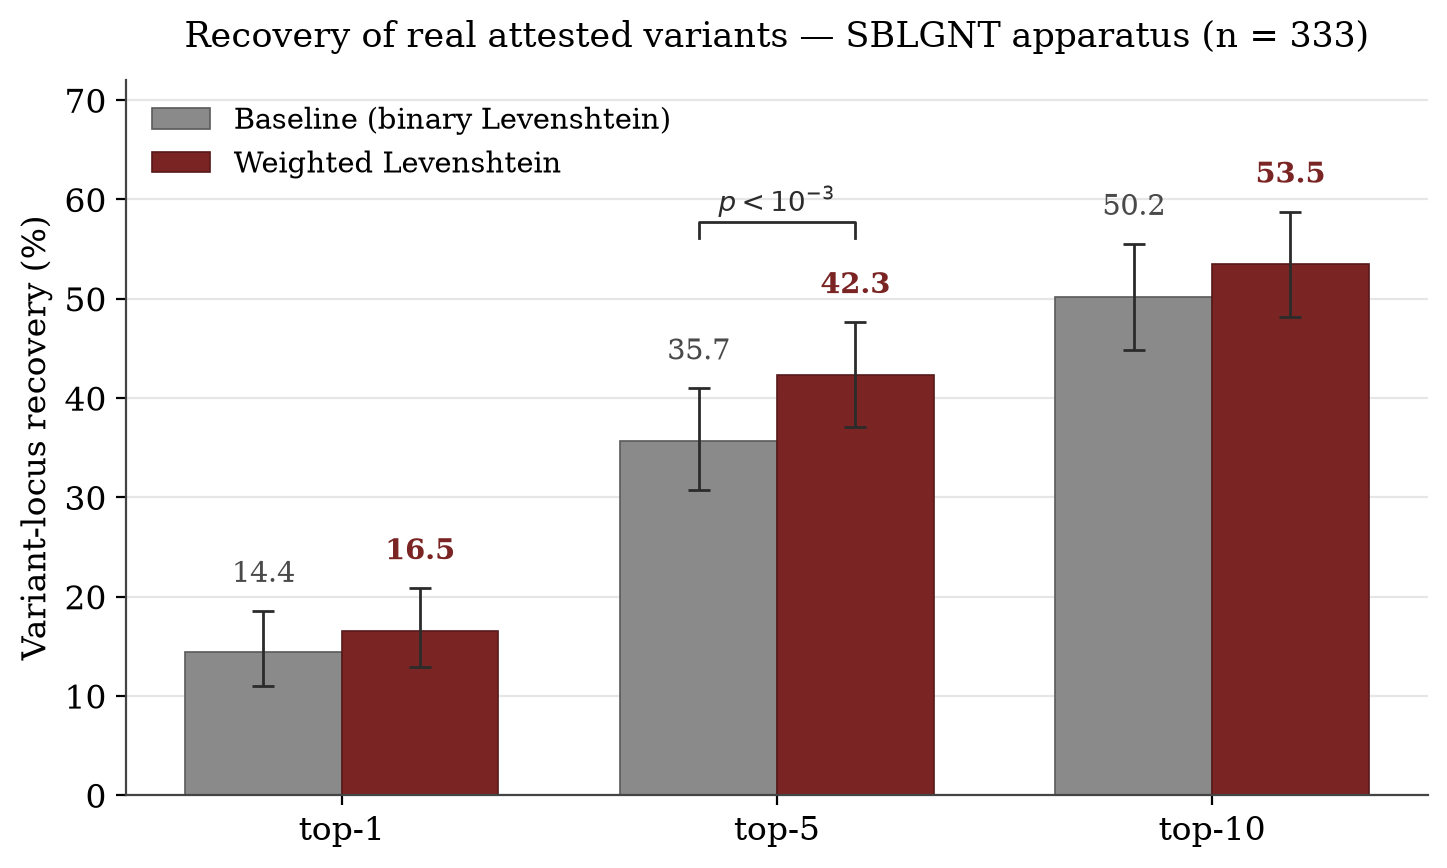
\includegraphics[width=0.92\linewidth]{fig_variants_topk.png}
  \caption{Real attested-variant recovery on SBLGNT ($n=333$). Recommended =
  weighted Levenshtein only. Error bars are Wilson $95\%$ confidence intervals;
  the top-5 gap is statistically significant.}
\end{figure}

The same direction appears in two more controlled tests. On the paper's
synthetic protocol ($n=200$), removing the weighted filter costs $-4.0$pp at
top-1 (one-tailed McNemar $p = 0.029$). On a corruption protocol built to mimic
scribal-class errors, removing it costs $-4.0$pp at top-10 ($p = 0.039$).

\section{What helped, what didn't}

Two further components were tested alongside the weighted distance. Both proved
to be dead weight, and the all-on combination does \emph{worse} than baseline
($-1.5$pp top-1, $-3.5$pp top-5).

\begin{table}[h]
  \centering
  \caption{Per-component ablation on artificial single-character corruption
  ($n=200$, \S4.1 protocol).}
  \begin{tabular}{lrrrr}
    \toprule
    Condition & Top-1 & Top-5 & Top-10 & McNemar $p$ \\
    \midrule
    Baseline (paper)        & $37.5\%$ & $69.5\%$ & $81.5\%$ & --- \\
    $-$CF temperature       & $37.5\%$ & $69.0\%$ & $80.0\%$ & $1.00$ \\
    \textbf{$-$Weighted Lev}& $\mathbf{33.5\%}$ & $67.5\%$ & $80.5\%$ & $\mathbf{0.057}$ \\
    $-$Extras (E1--E4)      & $37.0\%$ & $68.0\%$ & $81.5\%$ & $1.00$ \\
    All improvements        & $36.0\%$ & $66.0\%$ & $79.0\%$ & $0.63$ \\
    \bottomrule
  \end{tabular}
\end{table}

\begin{itemize}
  \item A \textbf{chance-fit adaptive temperature} (flatten the model's
  distribution when the written word is implausible) is inert --- an exact tie
  with baseline at top-1, McNemar $p = 1.00$.
  \item Four \textbf{extras (E1--E4)} are actively harmful on the realistic
  protocol: removing them lifts top-1 from $26.5\%$ to $30.5\%$ ($p = 0.021$).
  The likely culprit is the \emph{lectio difficilior} penalty (E1), which
  discounts suggestions more common than the written word --- exactly the pattern
  when an itacism slip moves a rare spelling to a common one.
\end{itemize}

The winning configuration is therefore the simple one: \textbf{weighted
Levenshtein on, everything else off.}

\section{Out-of-corpus deployment: Photius}

The system was then run on $26$ paragraphs (\textasciitilde$2{,}100$ words) of
Photius's \emph{Bibliotheca} (codices 70, 92, 161, 165, 213), a text outside
Logion's training corpus and surviving in two manuscript families (Marcianus gr.
450 and 451). Its shortlist clusters in the itacism and visual-confusion region,
as expected, but none of its picks align with documented apparatus loci. They are
best read as positions where the model and the transmitted text most diverge, not
as a curated emendation set.

\section{Caveats}

\begin{itemize}
  \item \textbf{Domain shift.} The public checkpoint is fine-tuned on Psellus
  (11th c.\ Byzantine). The variant test uses Koine (1st c.) and the Photius run
  is 9th c., so absolute accuracy sits below the paper's in-domain $90.5\%$. The
  relative deltas --- baseline vs.\ weighted on the same loci --- still hold.
  \item \textbf{The synthetic protocol is rigged against weighting.} It draws
  corruptions uniformly across the 24-letter alphabet, which quietly rewards an
  algorithm that treats every edit as equally likely. Weighting exists to exploit
  the non-uniform reality of scribal error, so the real-variant test is the one
  that counts.
  \item \textbf{A variant is not always an error.} Many SBLGNT variants are
  disagreements between defensible readings, not slips. The test measures whether
  Logion finds a locus unusual, which is weaker than asking whether it is wrong.
  \item \textbf{The weights are hand-tuned} from textbooks. The natural next step
  is to learn the phonetic prior from Byzantine palaeographic data, or to retrain
  the model with the weighted neighborhood as a training signal rather than only
  an inference-time filter --- which could internalize scribal error patterns
  directly and yield a larger gain.
\end{itemize}

\vspace{1em}
\noindent\footnotesize Built on Logion (Cowen-Breen et al., \emph{ACL
ALP-2023}). SBLGNT apparatus from \texttt{jjmccollum/sblgnt-tei} (CC BY 4.0).
Source: \texttt{github.com/Zed-Rez/logion-wlev}.

\end{document}
